\documentclass{article}
\usepackage{graphicx}
\graphicspath{ {images/} }
\usepackage[letterpaper, portrait, lmargin=1in, rmargin=1in, tmargin=1in, bmargin=1in]{geometry}

\title{External Validity of Experimental Social Preference Games}
\author{Sarah Xu}
\date{4 December 2017}

\begin{document}

\maketitle

\section{Introduction and Literature Review}

The standard economic model assumes actions are motivated purely by self-interest. However, it\rq s clear from simple observation that people actually care about the wellbeing of others: social programs exist, people volunteer, and people donate. If someone is not solely motivated by material self-interest but also cares positively or negatively for the material payoffs of others, we say that the person has social preferences. The last few decades have seen a strong surge of interest in this topic, with numerous research studies providing evidence of social preferences. Papers have identified different aspects of social preferences such as altruism, social welfare, inequality aversion, and reciprocity (e.g., Charness and Rabin 2000; Fehr and Schmidt 1999; Andreoni and Miller 2002; Rabin 1993; Fisman, Jakiela, and Kariv 2014). \\
 
When studying social preferences, the typical approach is to conduct experiments in a laboratory setting. There are many advantages to this approach. The experimental games allow researchers to target the different aspects of social behavior, and the laboratory setting strips the games from contextual features. This allows ceteris paribus observations of actions to be identified. For example, Fehr and Schmidt (1999) used ultimatum and dictator games to identify whether people have inequality aversion, Berg et al (1995) employed trust games to provide evidence of reciprocity, and Hermann, Thoni, and Gachter (2008) used public goods game to provide evidence of punishment and reciprocity. With thousands of other studies using various experimental games in a laboratory setting, this approach has become one of the building blocks of experimental and behavioral economics. \\
 
However, experiments conducted in the lab also has its disadvantages. They are abstract and remote from the real life experiences of subjects. Therefore, an important question is the extent to which the experimental games approach to social preferences can be generalized to real world situations. In practical scenarios, human behavior may be sensitive to a variety of factors not present in a lab setting. One issue is that in a lab setting, the subject's actions are under the scrutiny of the researcher. There is evidence that subjects in laboratory environments might alter their actions to conform to the behavior that they believe the experimenter desires. Benz and Meier (2006) compare how individuals behave in donation laboratory experiments with how the same individuals behave in the field, and find that subjects who have never donated in the past gave 60\% of their endowment in the lab experiment. This concern is also supported by other evidence that subjects are sometimes more prosocial in the lab than they are in the field (List, 2006; Gneezy et al., 2004). People are also influenced heavily on the context of the situation. Ross and Ward (1996), Burnham, McCabe, and Smith (2000), and Gintis (2001) find that slightly changing the narrative could result in significant changes in behavior. Stakes are also different between experimental games and natural situations. Carpenter, Verhoogen, and Burks (2005), Slonim and Roth (1998), and Parco, Rapoport, and Stein (2002) find that higher stakes leads to significantly different results than with lower stakes. Levitt and List (2007) point out a number of other differences between laboratory settings and naturally occurring situations.\\
 
The fact that varying factors such as scrutiny, context, and stakes can yield significant differences in behavior calls into question the external validity of using experimental games in a laboratory setting to study social preferences. There are some studies that have examined how people\rq s behavior in a lab setting is compared to the same people\rq s behavior in a naturally occurring situation, yielding mixed results. Baran et al (2010) compared MBA alumni donations to their university with their reciprocity behavior obtained in playing a trust game in the lab. They find that responder behavior in the trust game predicts the amount donated to the university. Franzen and Pointner (2013) compare behaviors from university students participating in standard dictator games and their actions when receiving a misdirected mail containing money. The authors find that subjects who showed other-regarding behavior in the lab returned the misdirected letters more often than subjects giving nothing, suggesting that in-lab behavior is related to behavior in the field. Englmaier and Gebhardt (2010) conducted field experiments with university students, comparing free riding behavior at the university library with free riding behavior when participating in a public goods experiment. The authors find statistically significant correlation between field and lab measures. There are also studies using non-student subjects. Fehr and Leibbrandt (2011) conducted public goods games with Brazilian fishermen, and find that fishermen who are more cooperative and more patient in the games were also less likely to exploit the communal fishing grounds in their daily lives. Karlan (2005) compared Peru inhabitants\rq  \ trust game behaviors to their repayment behavior of micro loans, and finds correlated behavior. \\

On the other hand, there are a number of papers that find play in lab experiments has no predictive power for behavior in naturally occurring settings. Goeschl et al (2015) examined university students\rq \ behavior in two different tasks: a public goods game and their contributions to a task directly linked to the reduction of CO2 emissions. The authors find that behavior in both tasks is uncorrelated. Hill and Gurven (2004) carried out ultimatum and public goods games on Paraguay Ache Indians. They compared the behaviors to observed food production and sharing patterns to individuals outside the nuclear family and found no significant relationships to lab behavior. Gurven and Winking (2008) used Tsimane forager-horticulturalists in Bolivia as their subjects, and compared behavior when playing dictator and ultimatum games to their food-sharing behavior. The authors find no relation between the two measures. Voors et al (2012) use a sample of subsistence farmers in Sierra Leone to compare behavior in a public goods game and behavior when asked earlier to contribute to a real community public good. They find no meaningful correlation in behavior across contexts. With other studies finding statistically significant, not statistically significant, and mixed results, we can see that the currently accumulated evidence is ambiguous. This is clear evidence that justifies further research is needed. \\

 
While the literature on the correlation between behavior of a single individual in both the lab and the field is growing, Galizzi and Navarro-Martinez (2017) argue that the studies only report the results of comparing one social preference game with one specific field measure. The abstract and context-free nature of experimental games makes it very difficult to establish clear theoretical correspondences between the games and real social behaviors outside the lab, and so it is crucial to conduct more systematic research on the external validity of social preference games. The authors proceed to carry out their own study, comparing behavior in different games with several behaviors elicited in the field and with self-reported behaviors exhibited in the past. Participants answered a set of questions about social behaviors exhibited in the past, played a variety of social preference games in a laboratory, and encountered naturalistic situations related to social preferences in the field. Examples of the field situations included a research assistant asking for help carrying boxes to the basement of the university building where the lab was located, asking to use the participant\rq s phone to make a brief phone call, asking for donations to a children\rq s charity, asking for donations to an environmental charity, or asking for donations to the lab\rq s research fund.  Their overarching conclusion is that the games do a poor job explaining both the self-report measures and the field behaviors, although more systematic studies are needed to draw a definite conclusion. For example, future studies could look at other field situations or other game structures. \\

It is critical to think about why some experiments found correlations and some did not, in order to inform the design of our current experiment. An underlying theme for those experiments that found no correlations is higher stakes. Voors et al (2012) note that an important difference between the lab and field experiment are that the stakes are much higher in the field experiment: a month of wages versus a day\rq s wage, and the public good affected the entire village instead of two other co-players. In Gurven and Winking (2008)\rq s study, there are different stakes between the experimental and field measures. The authors note that ``money is fungible and easier to hide than agricultural produce or meat and is shared differently than other resources''. In addition, stakes are especially higher for food-sharing behavior since food-sharing is heavily ingrained in the culture. Lastly, while playing the experimental games for Hill and Gurven (2004)\rq s study, participants expressed worry that their choices would make the receiver upset. In particular, the tribal group\rq s culture was heavily focused on community, and was well known for extensive food sharing (which was the field measure the authors used). Perhaps the participants didn\rq t want to risk their choices creating any tension in their community, and getting punished with less food sharing and cooperation. For the last two papers, the stakes were a result of high scrutiny and low anonymity since it was easy for community members to find out the choices each subject made. For our design, an important aspect is that participants will play the games in their own time and location to ensure no scrutiny and high anonymity. \\

Similar to Galizzi and Navarro-Martinez (2017), I will recruit Wesleyan University students to play various experimental games and non-incentivized social preference questions.  A major criticism of the design is how the authors executed their field measures. Since the setup occurs as the participants are exiting their lab session, it\rq s hard to believe that the participants did not connect the encounters to the research lab, especially since they previously answered questions similar to the current event. Therefore it is better to use a natural, far-removed situation. For my paper, I will be using donations of seniors and recent alumni to Wesleyan University. Donors can choose what area their donations will go towards (for example financial aid, academic programming and faculty support, and or student activities). These different donation options can be related to some behavioral constructs. For example, donating may represent altruism and reciprocity, and donating to financial aid may represent inequality aversion. \\
 
Along with adding to the literature on external validity of experimental social preference games, there is a potential policy implication with our findings. It will be interesting to see whether experimental games or survey/hypothetical questions better predict behavior in the real world. Experimental games are costly - not only is it expensive paying participants for attending the lab session and providing money aligned with the payoffs of the games (especially if more show up than expected), but it also takes a lot of time to program the experimental games. If experimental games do not better predict field measures, then perhaps eliminating experimental games and instead using non-incentivized survey questions is better for funding and logistical purposes. Therefore the overarching goal is to determine which model can better predict social preferences exhibited in the field. \\
 
        	Ultimately, I hope my paper will add to the growing literature on the external validity of experimental social preference games. By comparing my results with those of past studies, I can contribute to the discussion on whether experimental games are a useful tool to examine social preferences. In addition, my paper can perhaps spark interest into future studies into the external validity of other behavioral economics topics where lab experiments are commonly used. \\


\section{Methods}

Our goal is to evaluate the external validity of experimental social preference games to behaviors in the field. We will be presenting the same sample of participants with two sets of tasks: (1) survey questions regarding past social behavior, and (2) incentivized social preference games. The field measure that we will be comparing their results to is their donations to Wesleyan. \\
 
Both instruments will be sent via a single link in an email, and participants will be able to play the experimental games and answer the survey and non-incentivized questions online remotely (images of the computerized games and questions are in Figure 1). \\
 
The participants will receive a unique identifier, as well as detailed instructions for the tasks they will complete throughout their session. They will then be told that, upon their permission, their Wesleyan donations information will be released to us. They will be informed that their information will be linked to their unique identifier, and only the researchers involved will have access to the information. \\


\subsection{Self-reported measures of past social behaviors}

Participants reported on their past social behaviors using questions loosely based off of the Self-Report Altruism (SRA) scale introduced by Rushton, Chrisjohn, and Fekken (1981). \\

The scale consists of 20 items, and participants report how frequently in the past they have done different actions related to social behaviors. Participants rated each statement on a scale from 1 (``never'') to 5 (``very often''). Examples include: ``I have donated money at the cash register when buying groceries'', ``I have pointed out a clerk\rq s error (at the supermarket, at a restaurant) in undercharging me'', and ``I have donated instead of sold my clothes/used items''. A full list of the 20 items is contained in Table 1. \\

\subsection{Incentivized social preference games}

Participants also play various social preference games. Since they are completing the games at their own availability, they will not be randomly matched up with other participants. Instead, if the game requires two players, the second player will see a list of all possible options, and are prompted for their choice for each option listed (further discussion about the strategy method is in Section 2.2.1). \\

I will use five games that are widely used in behavioral economics to study social preferences: dictator game, generalized dictator game, ultimatum game, trust game, and public goods game. There will be different variations of each game (each participant will play the role of Player 1 (the proposer) and Player 2 (the responder)), and all the games are independent from each other. If the participant is Player 2, they are given a list of possible options, and are prompted to make a decision for each option that is listed. At the end, one of the games is randomly selected and the participants are paid the amount they earned in that particular game. All the games are computerized, and they were programmed and implemented using oTree. \\

Participants first receive instructions on the various games and the general payment mechanism. They will be told that payoffs are represented in experimental currency units (ECU), and that 10 ECU equals \$1. They will be informed that after they have completed all the games, one game will be randomly picked. Their answers will be randomly matched with other players, and payoffs will be calculated for that game. Payoffs will then be translated into US dollars, and they will receive their payment via PayPal.\\

Below are the different games: \\

\begin{enumerate}

\item Dictator Game: Each participant decides how to divide 10 ECU between themselves and an anonymous, random Player 2.
\item Generalized Dictator Game:  Each participant (playing as Player 1)  is asked to make a series of choices about how to divide points between themselves and an anonymous, random Player 2. As Player 1 divides the points, both players will each earn money. Every point that Player 1 earns will be worth 10, 20, 30 or 40 cents, depending on the choice. Similarly for the earnings of Player 2. The design is based off of Andreoni and Miller (2002).
\item Ultimatum Game Player 1: Each participant is endowed with 10 ECU. They decide how much of their endowment to send to an anonymous, random Player 2. They are told that Player 2 may or may not reject the allocation. If the allocation is rejected, both players receive 0 ECU.
\item Ultimatum Game Player  2: Each participant is now the responder (Player 2). They are given a list from 1 ECU to 10 ECU (in 1 ECU increments), and are asked whether they accept or reject each listed amount.
\item Trust Game Player 1: Each player is endowed with 10 ECU. They decide how much of their endowment to send to an anonymous, random Player 2. The amount sent over is multiplied by three. Player 2 then decides how much to return. 
\item Trust Game Player 2: Now each players is the responder (Player 2). They receive a list of all ten possible multiplied amounts that Player 1 could have chosen to send, 0 to 3x. For each amount, they are prompted to enter the amount they would like to return.
\item Public Goods Game: Each participant is endowed with 10 ECU and have to decide how much of their endowment to contribute to a common group fund with three other anonymous, random participants. The overall money in the group is multiplied by two and divided evenly between the four players.

\end{enumerate}

Note that since participants will be playing the games in their own time, they will not be paired up with other people. Instead, they will be paired up randomly at the time payments will be calculated. We will explain the payment process in the next section. \\
 
These experimental games cover a substantial proportion of research on social preferences and they address many of the main behavioral constructs invoked in the literature to explain social behaviors. Some constructs include: altruism (dictator game, public goods game); positive reciprocity (trust game  responder); negative reciprocity (ultimatum game responder); trust (trust game proposer); cooperation (public goods game); and inequality aversion (all games). 

\subsubsection{Strategy Method}

Each participant has the opportunity to be both proposer (Player 1) and responder (Player 2) in each game. When the participant is the responder, we use the strategy method: the participant has to make decisions for all possible situations. For example, as the responder in the trust game, the participant has to decide how much money they will send back for all possible amounts that were given to them by the proposer. \\

There are several reasons why we use the strategy method. First, as mentioned previously, participants complete the experimental games in their own time, so participants will not be paired up while they are playing. Instead, they will be randomly paired at a later period. Therefore it is useful to have all of Player 2\rq s potential choices so that payoffs can be determined. Most importantly, the strategy method gives more information. If participants were to be matched at the time they were playing the games, then we would only get information on how much the responder will give back for the one amount that the proposer donates. Using the strategy method will allow us to see all returned amounts for all possible donated amounts in the ultimatum game, and we can also see the minimum donated amount that the responder will accept in the trust game. \\

\subsubsection{Payment}
At the end of the deadline, one game will be randomly picked for payment. Players will be randomly matched for the game. Below are the descriptions of how payoffs will work for each game: 

\begin{enumerate}

\item Dictator game: Participants will be paired up randomly. In each pair, one player will be randomly selected as the dictator, and the other will be the receiver. The dictator will receive their endowment minus their offer amount, and the receiver will receive the offer amount.

\item Generalized dictator game: Participants will be paired up randomly. In each pair, one player will be randomly selected as the dictator, and the other will be the receiver.  Since the generalized dictator game consisted of 10 different sets of endowment and prices, one will be picked for payment. For the chosen set, the dictator will receive their endowment minus their offer amount, and the receiver will receive the offer amount (both adjusted according to the hold and pass prices).

\item Ultimatum game: Half of the participants will be randomly assigned to their Player 1 choices (Ultimatum game 1), and the other half will be assigned to their Player 2 responses (Ultimatum game 2). They will then be randomly matched, and payoffs will be determined. For example, if Player 1 chose to give 4 ECU but Player 2 chose not to accept that amount, then both players will receive nothing. But if Player 2 does accept that amount, then Player 1 will receive 6 ECU and Player 2 will receive 4 ECU.

\item Trust game: Half of the participants will be randomly assigned to their Player 1 choices (Trust game 1), and the other half will be assigned to their Player 2 responses (Trust game 2). They will be randomly paired up, and payoffs will be determined. For example, if Player 1 chose to give 2 ECU to Player 2, then the multiplied amount is 6 ECU. Given being offered 6 ECU, if Player 2 chose to give back 1 ECU, then ultimately Player 1 will receive 9 ECU and Player 2 will receive 5 ECU.

\item Public goods game: Participants will be randomly assigned to groups of four. The overall money in the pool will be multiplied by two and divided evenly. Thus each participant will receive their remaining amount plus the divided pooled amount from the pool.

\end{enumerate}

Each player will receive their payoffs in US dollars. They will receive their payments via PayPal.


\subsection{Field Measure}

Each participant\rq s Wesleyan donations information will be accessed upon their informed consent and completion of the survey and games. \\

Wesleyan donations can represent different aspects of social preferences. Whether a participant donates or not can represent altruism. Donating can also represent reciprocity, since seniors/recent alumni are giving back to the university that provided them four years of education and opportunities, as well as represent cooperation and trust. In addition, donors are able to target what area their donations can go towards. For example, donating towards Financial Aid can represent inequality aversion, since Financial Aid makes the Wesleyan experience possible for talented, low-income students who might not otherwise be able to attend.  \\

	A main feature of our design is that the donations information is a naturalistic environment that is far-removed from the experiment. We believe that this is a more accurate field measure. We previously mentioned that Galizzi and Navarro-Martinez (2017)\rq s design is unsatisfactory since their subjects encountered the field experiment shortly after completing the lab experiments. We believe that it is not too difficult to link the two situations together. In our design, participants\rq \ donations behavior is not affected by their participation in the lab at the time.
	
\subsection{Participants and Sessions}
Emails containing the link to access the online experimental games and survey questions will be sent to all current Wesleyan University seniors and recent alumni (those who graduated within 5 years) in early January. They will have until mid-February to participate. The participants are those who volunteer to open the email link, provide consent for us to access their Wesleyan donations data, and complete both the survey questions and social preference games. Besides soliciting seniors and recent alumni to participate, we use no other eligibility or exclusion criteria to select participants.

\section{Analysis}

After gathering all experimental, survey, and donations data, we will be running two regression models:

\begin{equation}
donations= \beta_{0} + \beta_{1} DG + \beta_{2} GDG + \beta_{3} UG1 + \beta_{4} UG2 + \beta_{5} TG1 + \beta_{6} TG2 + \beta_{7} PGG
\end{equation}

\begin{equation}
donations = \beta_{0} + \beta_{1} SRA
\end{equation}

where DG = dictator\rq s pass rate (percentage of the initial endowment of points passed to the other player) in the dictator game, GDG = dictator\rq s pass rate in the generalized dictator game, UG1 = proposer\rq s pass rate in the ultimatum game, UG2 = proposer\rq s minimum pass rate that the responder choose to accept in the ultimatum game, TG1 = proposer\rq s pass rate in the trust game, TG2 = responder\rq s return ratio for each possible donated amount in the trust game, PGG = player\rq s pass rate into the public pool, and SRA = participant\rq s self-report altruism score. \\

First, we will run each model and examine how well each instrument predicts donations. With Model (1), we want to see which game best predicts donations behavior. For example, if we see that the dictator game and responder ultimatum game is statistically significant but all other games are not statistically significant, then perhaps further research could exclude using the other games when predicting charitable giving. This would certainly save researchers the time cost in programming the games, as well as make the experiment shorter (and therefore more attractive to participants). \\

However, our overall goal is to determine whether results from incentivized experimental games or non-incentivized self reported measures can better predict field measures on social preferences. Therefore we want to examine the prediction errors in order to conclude which model is better. 


\appendix
\section{Tables}

\begin{tabular}{ | p{12cm} | }
\hline
\multicolumn{1}{|c|}{SRA Questions List} \\
\hline
1. I have delayed an elevator/held door open for stranger(s).\\
\hline
2. I have given directions to a stranger.\\
\hline
3. I have gone out of my way to meet with someone to help them with a task (e.g. help proofread their paper, listen to their presentation, etc).\\
\hline
4. I have donated money at the cash register when buying groceries.\\
\hline
5. I have given money to a stranger (or an acquaintance I don?t know too well) in need.\\
\hline
6. I have donated instead of sold my clothes/used items.\\
\hline
7. I have donated to a charity.\\
\hline
8. I have donated blood.\\
\hline
9. I have done volunteer work for a charity/organization.\\
\hline
10.  I have signed an online petition / shared a cause on social media.\\
\hline
11. I have allowed someone to go ahead of me in line.\\
\hline
12. I have lent an acquaintance that I don?t know too well with something of value to me (clothes, tools, etc).\\
\hline
13. I have pointed out a clerk\rq s error (at a supermarket, restaurant) in undercharging me.\\
\hline
14. I have let an acquaintance that I don?t know too well stay at my place.\\
\hline
15. I have donated money/coins into Salvation army bell-ringers.\\
\hline
16.I have helped a classmate who I did not know that well with a homework assignment when my knowledge was greater than his/hers.\\
\hline
17. I have offered to give a ride to someone without asking to be paid for it.\\
\hline
18.  I have helped carry a stranger\rq s belongings (e.g. groceries).\\
\hline
19. I have offered my seat on a bus/train to a stranger who was standing.\\
\hline
20. I have helped an acquaintance with moving in/ moving out of their dorm/apartment/house.\\
\hline
\end{tabular}



\section{Figures}
Figure 1: Online games and survey questions \\
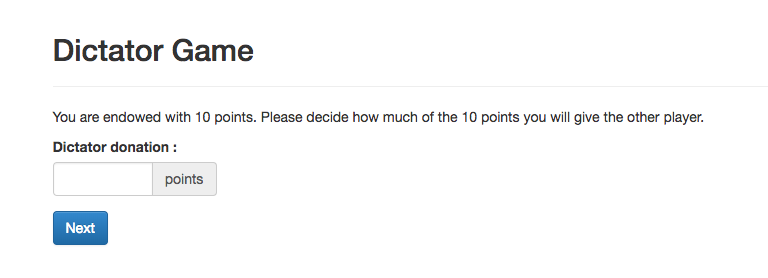
\includegraphics[scale=0.5]{dictator} \\
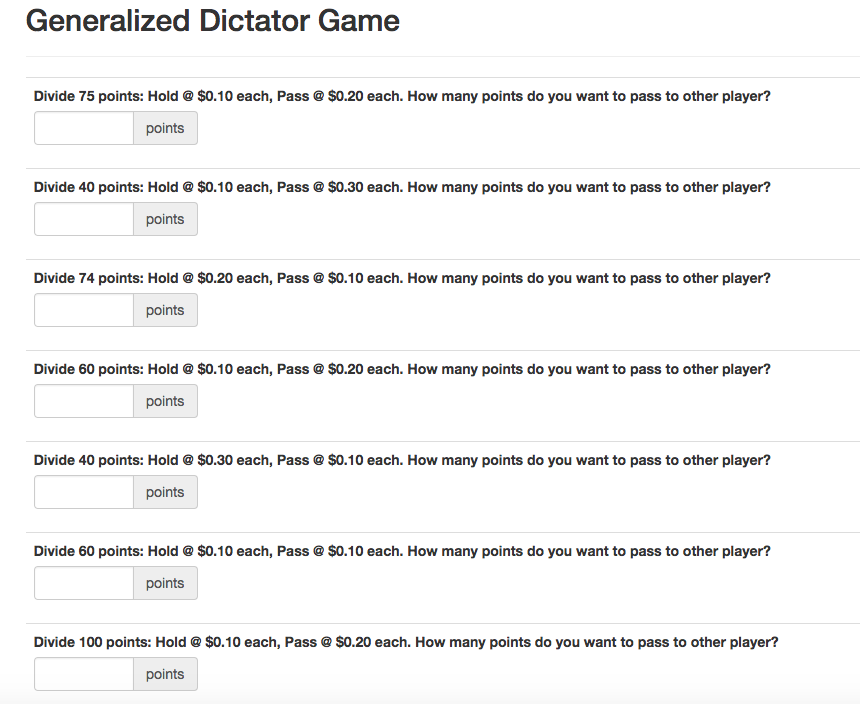
\includegraphics[scale=0.5]{generalized_dictator} \\
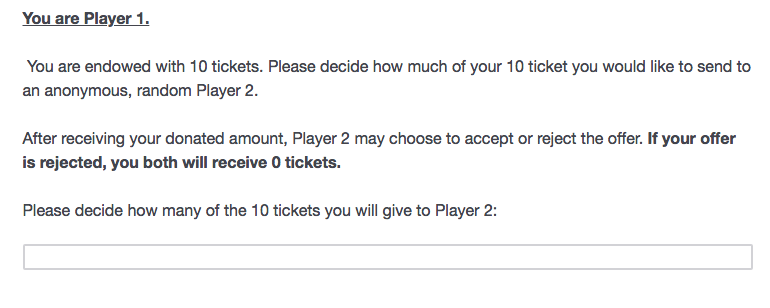
\includegraphics[scale=0.5]{ultimatum1} \\
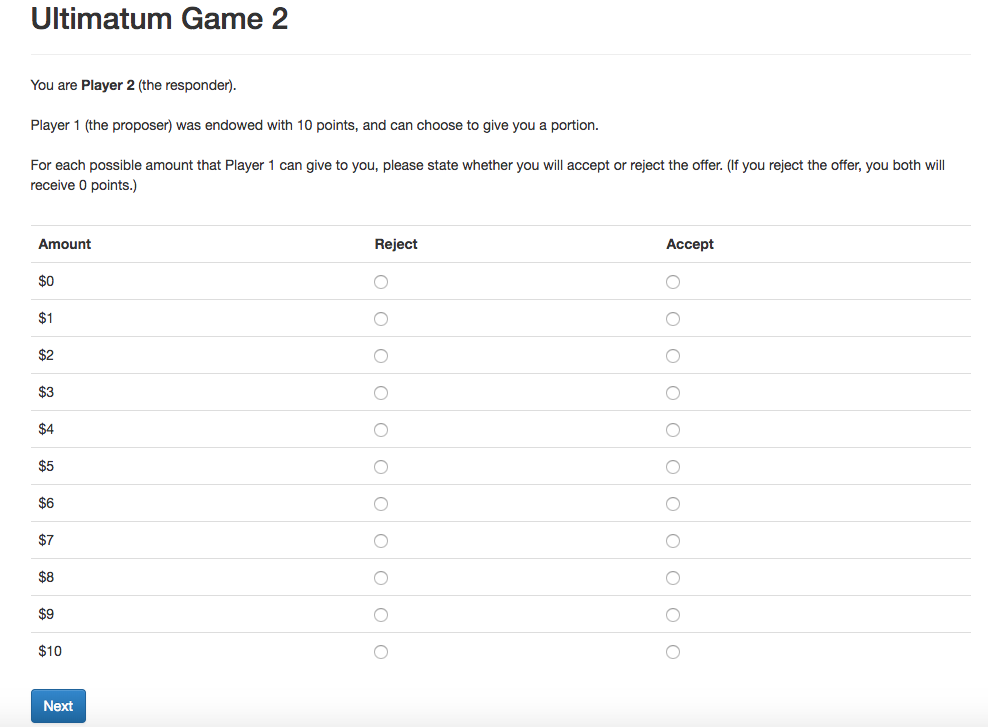
\includegraphics[scale=0.5]{ultimatum2} \\
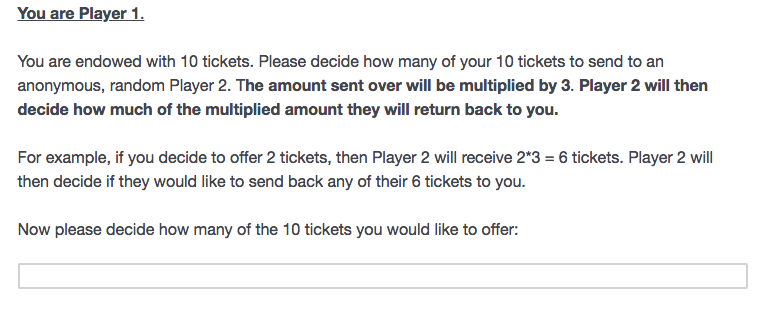
\includegraphics[scale=0.5]{trust1} \\
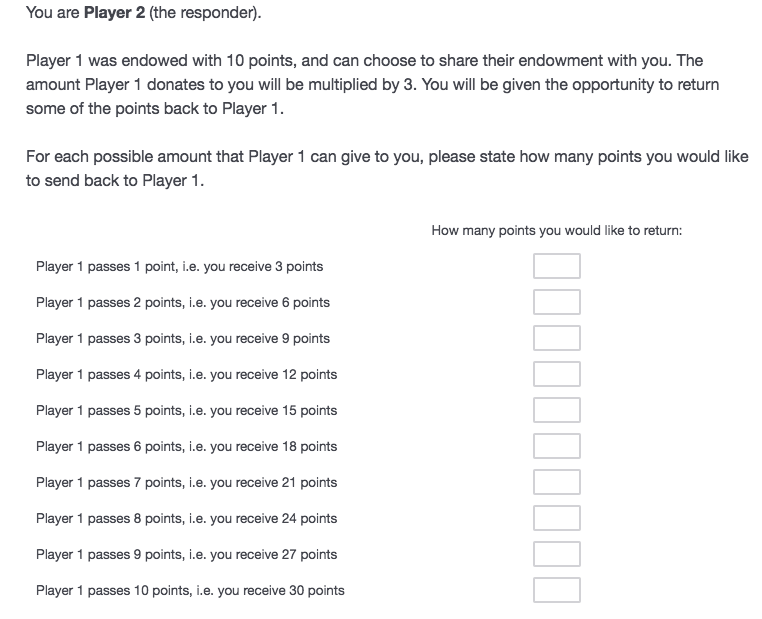
\includegraphics[scale=0.5]{trust2} \\
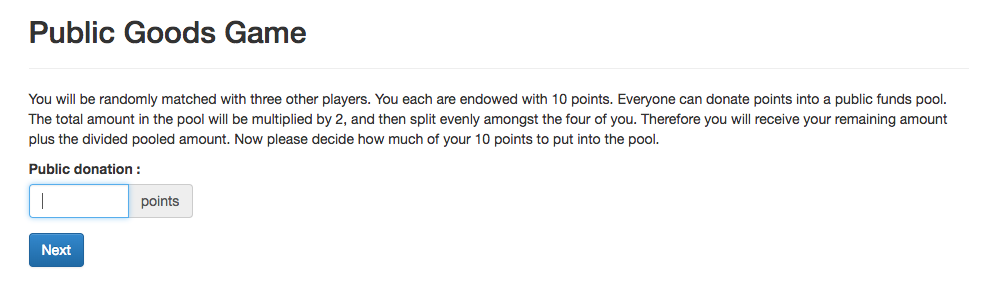
\includegraphics[scale=0.5]{public} \\
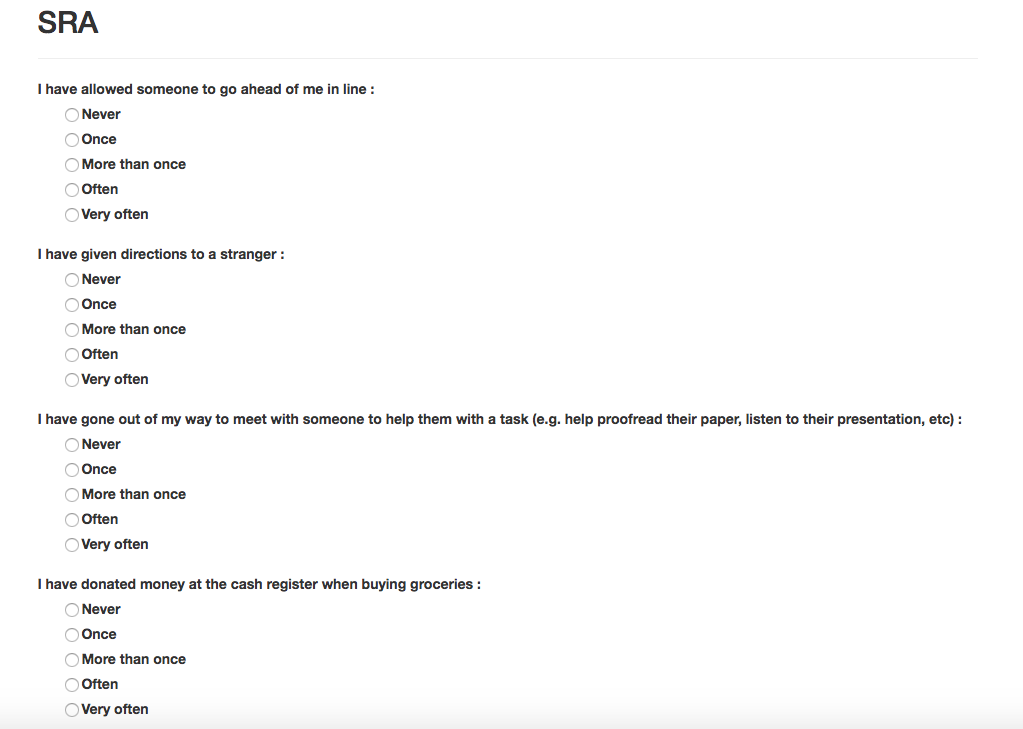
\includegraphics[scale=0.5]{sra} \\


\begin{thebibliography}{9}

\bibitem{AndreoniMiller}
Andreoni, J., and Miller, J.H. (2002).
\textit{Giving according to GARP: An experimental test of the consistency of preferences for altruism}.
Econometrica, 70, 737-53.

\bibitem{Baran}
Baran, N.M., Sapienza, P., and Zingales, L. (2010).
\textit{Can we infer social preferences from the lab? Evidence from the trust game}.
NBER Working Paper 15654.

\bibitem{Benz}
Benz, M., and Meier, S. (2006).
\textit{Do people behave in experiments as in the field? Evidence from donations}.
Experimental Economics, 11, 268-81.

\bibitem{Berg}
Berg, J., Dickhaut, J.W., and McCabe, K.A. (1995).
\textit{Trust, reciprocity, and social history}.
Games and Economic Behavior, 90, 166-93.

\bibitem{Burnham}
Burnham, T., McCabe, K., Smith, V. (2000).
\textit{Friend-or-foe intentionality priming in an extensive form trust game}.
Journal of Economic Behavior \& Organization, 43, 57-73.

\bibitem{Carpenter}
Carpenter, J.P., Verhoogen, E., and Burks, S. (2005).
\textit{The effect of stakes in distribution experiments}.
Economics Letters, 86, 393-98.

\bibitem{CharnessRabin}
Charness, G., and Rabin, M. (2002).
\textit{Understanding social preferences with simple tests}.
Quarterly Journal of Economics, 117, 817-69.

\bibitem{Englmaier}
Englmaier, F., and Gebhardt, G. (2010)
\textit{The external validity of giving in the dictator gam: A field experiment using the misdirected letter technique}.
Governance and the efficiency of social systems (GESY), CESifo Working Paper No. 344.

\bibitem{FehrLeibbrandt}
Fehr, E., and Leibbrandt, A. (2011)
\textit{A field study on cooperativeness and impatience in the Tragedy of the Commons}.
Journal of Publicc Economics, 95, 1144-55.

\bibitem{FehrSchmidt}
Fehr, E., and Schmidt, K. (1999).
\textit{A theory of fairness, competition, and cooperation}.
Quarterly Journal of Economics, 114, 173-68.




\bibitem{Fisman}
Fisman, R., Jakiela, P., and Kariv, S. (2014).
\textit{The distributional preferences of Americans}.
NBER Working Paper.

\bibitem{Franzen}
Franzen, A., and Pointner, S. (2013)
\textit{The external validity of giving in the dictator gam: A field experiment using the misdirected letter technique}.
Experimental Economics, 16, 155-69.

\bibitem{Galizzi}
Galizzi, M., and Navarro-Martinez, D. (2017).
\textit{On the external validity of social preference games: a systematic lab-field study}.
Management Science.

\bibitem{Gintis}
Gintis, H. (2000).
\textit{Strong reciprocity and human sociality}.
Journal of Theoretical Biology, 206, 169-79.

\bibitem{Gneezy}
Gneezy, U., Haruvy, E., and Yafe, H. (2004).
\textit{The inefficiency of splitting the bill: A lesson in institutional design}.
The Economic Journal, 114(495), 265-80.

\bibitem{Goeschl}
Goeschl, T., Kettner, S.E., Lohse, J., and Schwieren, C. (2015)
\textit{What do we learn from public good games about voluntary climate action? Evidence from an artefactual field experiment}.
University of Heidelberg, Department of Economics Discussion Paper 595.

\bibitem{GurvenWinking}
Gurven, M., Winking, J. (2008).
\textit{Collective action in action: prosocial behavior in and out of the laboratory}.
American Anthropologist, 110(2), 179-190. 

\bibitem{Hermann}
Hermann, B., Thoni, C., and Gachter, S. (2008).
\textit{Anti-social punishment across societies}.
Science, 319, 1362-67.

\bibitem{HillGurven}
Hill, K., and Gurven, M. (2004)
\textit{Economic experiments to examine fairness and cooperation among the Ache Indians of Paraguay}.
In J. Henrich, R. Boyd, S. Bowles, C. Camerer, E. Fehr, and H. Gintis (Eds.),
Foundations of Human Sociality: Economic Experiments and Ethnographic Evidence from Fifteen Small-Scale Societies. Oxford University Press.

\bibitem{Karlan}
Karlan, D.S. (2005).
\textit{Using experimental economics to measure social capital and predict financial decisions}.
American Economic Review, 95, 1688-99.

\bibitem{Levitt}
Levitt, S., and List, J. (2007)
\textit{What do laboratory experiments measuring social preferences reveal about the real world?}.
Journal of Economic Perspectives, 21(2), 153-74.


\bibitem{List}
List, John. 2006.
\textit{The behavioralist meets the market: measuring social preferences and reputation effects in actual transactions}.
Journal of Political Economy, 114(51), 1-37.


\bibitem{Parco}
Parco, J., Rapoport, A., and Stein, W. (2002).
\textit{Effects of financial incentives on the breakdown of mutual trust}.
Psychological Science.

\bibitem{Rabin}
Rabin, M. (1993).
\textit{Incorporating fairness into game theory and economics}.
The American Economic Review, 83, 1281-1302.

\bibitem{Ross}
Ross, L., and Ward, A. (1996).
\textit{Naive realism in everyday life: Implications for social conflict and misunderstanding}.
Values and Knowledge, 103-35.

\bibitem{Rushton}
Rushton, J.P., Chrisjohn, R.D., and Fekken, G.C. (1981).
\textit{The altruistic personality and the self-report altruism scale}.
Personality and Individual Differences, 2, 293-302.

\bibitem{Slonim}
Slonim, R., and Roth, A. (1998).
\textit{Learning in high stakes ultimatum games: An experiment in the Slovak Republic}.
Econometrica, 66, 569-96.


\bibitem{Voors}
Voors, M., Turley, T., Kontoleon, A., Bulte, E., and List, J.A. (2012).
\textit{Exploring whether behavior in context-free experiments is predictive of behavior in the field: Evidence from lab and field experiments in rural Sierra Leone}.
Economic Letters, 114, 308-311.


\end{thebibliography}

	
\end{document}